\question Os dados abaixo representam as vendas semanais, em classes de salários mínimos, de vendedores de gêneros alimentícios:
\begin{parts}
    \part Faça o histograma dos dados.
    \begin{solution}
        \begin{figure}[H]
            \centering
            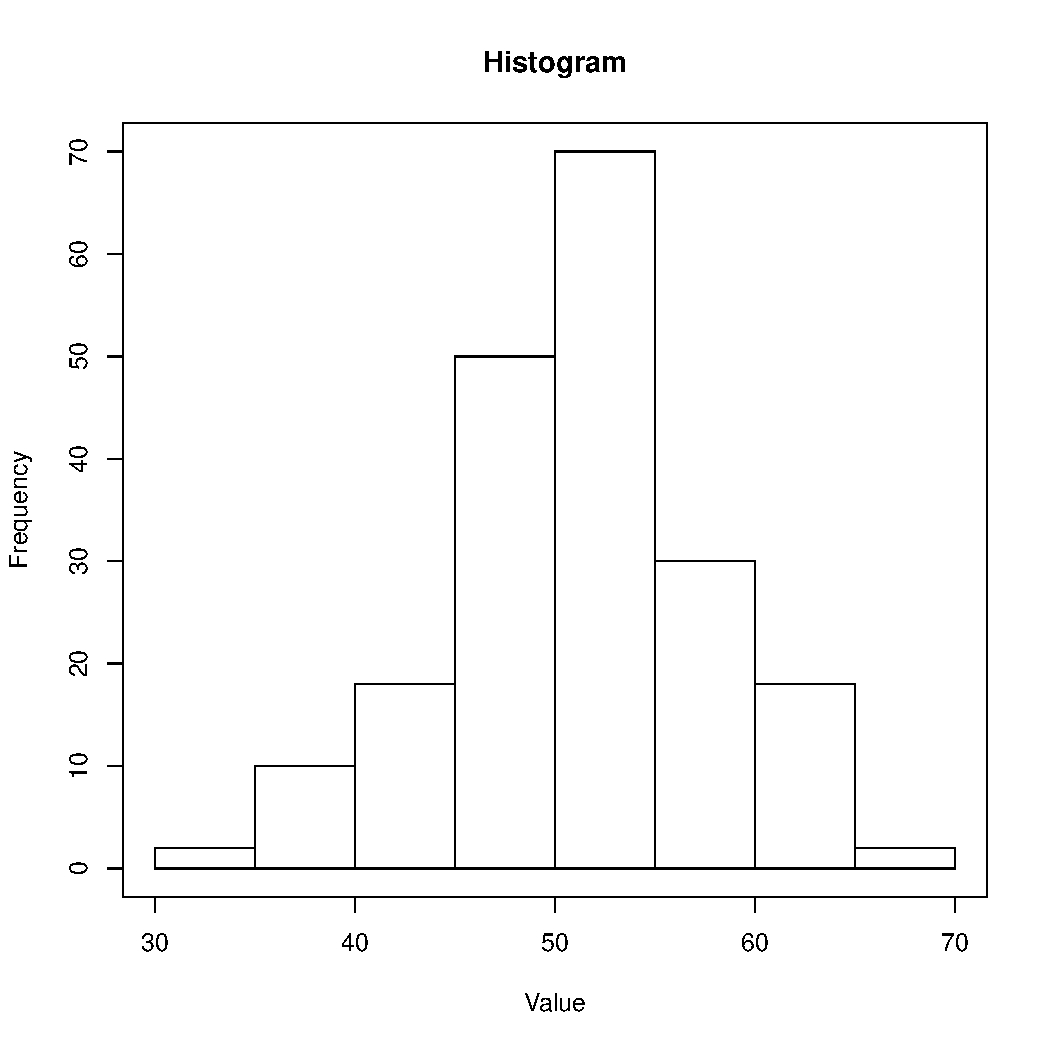
\includegraphics[width=8cm]{./../src/output/04092024_Output_BoxPlotVendasSemanais.pdf}
        \end{figure}
    \end{solution}

    \part Determine uma média amostral.
    \begin{solution}
        A média amostral nesse caso será dada pela média ponderada (sendo o \textbf{peso as frequências de cada classe}) dos pontos médios das classes, logo:
        \begin{equation*}
            \begin{split}
                \overline{x} & = \frac{\sum\limits^{k}_{i=1}{n_ix_i}}{n}, \text{onde } x_i \text{ é o ponto \textbf{médio da classe}}                                                         \\
                             & = \frac{\sum\limits^{8}_{i=1}{n_ix_i}}{200} = \frac{(2 \times 32.5) + (10 \times 37.5) + (18 \times 42.5) + (50 \times 47.5) + \dots + (2 \times 67.5)}{200} = \\
                \overline{x} & = \frac{10240}{200} = 51.2
            \end{split}
        \end{equation*}
    \end{solution}

    \pagebreak

    \part Prove que $\sum^k_{i=1}{n_i(x_i - \overline{x})^2} = \sum^k_{i=1}{n_ix^2_i} - n\overline{x}^2$, em que $k$ é o número de classes e $n_i$ a frequência simples da classe i.
    \begin{solution}
        \begin{proof}
            Dado que:
            \begin{equation*}
                \begin{split}
                    \sum^{k}_{i=1}{n_i(x_i - \overline{x})^2} \\
                \end{split}
            \end{equation*}
            Podemos expandir, assim:
            \begin{equation*}
                \begin{split}
                     & \sum^{k}_{i=1}{n_i(x^2_i - 2x_i\overline{x} + \overline{x}^2)} =                                   \\
                     & \sum^{k}_{i=1}{(n_ix^2_i - n_i2x_i\overline{x} + n_i\overline{x}^2)}                               \\
                     & \sum^{k}_{i=1}{n_ix^2_i} - 2\overline{x}\sum^{k}_{i=1}{n_ix_i} + \overline{x}^2\sum^{k}_{i=1}{n_i}
                \end{split}
            \end{equation*}
            Dado que a \textbf{frequência total é a soma das frequências}, ou seja, $\sum^{k}_{i=1}{n_i} = n$, temos que:
            \begin{equation*}
                \begin{split}
                     & \sum^{k}_{i=1}{n_ix^2_i} - 2\overline{x}\sum^{k}_{i=1}{n_ix_i} + \overline{x}^2n
                \end{split}
            \end{equation*}
            Outro fator é que temos que a \textbf{média em distribuições de frequência por classe} é dada por $\overline{x} = \frac{\sum^k_{i = 1}{n_ix_i}}{n}$, sendo $x_i$ a média da classe $i$, $n_i$ a frequência da classe $i$ e $n$ a frequência total, logo:
            \begin{equation*}
                \begin{split}
                    \overline{x} = \frac{\sum^k_{i = 1}{n_ix_i}}{n} \\
                    \therefore n\overline{x} = \sum^{k}_{i=1}{n_ix_i}
                \end{split}
            \end{equation*}
            Assim, temos que:
            \begin{equation*}
                \begin{split}
                     & \sum^{k}_{i=1}{n_ix^2_i} - 2\overline{x}n\overline{x} + \overline{x}^2n = \\
                     & \sum^{k}_{i=1}{n_ix^2_i} - 2\overline{x}^2n + \overline{x}^2n =           \\
                     & \sum^{k}_{i=1}{n_ix^2_i} - n\overline{x}^2
                \end{split}
            \end{equation*}
        \end{proof}
    \end{solution}

    \part Utilize a informação da parte (c) para determinar o desvio-padrão\footnote{Dado a variância, um valor normalmente expresso em casas ao quadrado, utilizamos o desvio-padrão que \textbf{faz a transformação dessa unidade (ao quadrado) para a original}} amostral ($s$).
    \begin{solution}
        Dado que o \textbf{desvio-padrão amostral} é dado por $s = \sqrt{\frac{1}{n-1} \times \sum^{k}_{i=1}{n_i(x_i - \overline{x})^2}}$, temos que:
        \begin{equation*}
            \begin{split}
                s & = \sqrt{\frac{1}{n-1} \times \Bigg[\sum^{k}_{i=1}{n_i(x_i - \overline{x})^2}\Bigg]} = \\
                  & = \sqrt{\frac{1}{n-1} \times \Bigg[\sum^{k}_{i=1}{n_ix^2_i} - n\overline{x}^2\Bigg]}
            \end{split}
        \end{equation*}
        Assim, com a fórmula atualizada façamos:
        \begin{equation*}
            \begin{split}
                s & =\sqrt{\frac{1}{199} \times \Bigg[\sum^{8}_{i = 1}{n_ix^2_i} - 200 \times 51.2^2\Bigg]}                                                                    \\
                  & = \sqrt{\frac{1}{199} \times \Bigg[((2 \times 32.5^2) + (10 \times 37.5^2) + (18 \times 42.5^2) + \dots + (2 \times 67.5^2)) - 200 \times 51.2^2 \Bigg]} = \\
                  & = \sqrt{\frac{1}{199} \times [533050 - 524288]} =                                                                                                          \\
                  & = \sqrt{44.03} =                                                                                                                                           \\
                s & \approx 6.63
            \end{split}
        \end{equation*}
    \end{solution}

    \pagebreak

    \part Qual a porcentagem das observações compreendidas entre $\overline{x} - 2s$ e $\overline{x} + 2s$?
    \ifprintanswers
        \savenotes
    \fi
    \begin{solution}
        Ambos serão interpretados como quantis, assim $Q_1 = \overline{x} - 2s$ e $Q_2 = \overline{x} + 2s$ e assim temos $Q_1 = 37.94$ e $Q_2 = 64.46$.

        A partir disso podemos utilizar a \textbf{fórmula de quantis em distribuições de frequência por classe}, isto é $Q_p = l_i + \frac{h(p - F_{i - 1})}{f_i}$\footnote{$p$ sendo a \textbf{proporção de observações menores ou iguais ao quantil desejado}}, para isso é interessante ter a tabela com as informações da \textbf{frequência relativa e relativa acumulada}, assim:

        % latex table generated in R 4.3.3 by xtable 1.8-4 package
        % Mon Apr  8 22:45:37 2024
        \begin{table}[H]
            \centering
            \begin{tabular}{rrrr}
                \hline
                Classe & freqAcum ($N$) & freqReq ($f$) & freqRelAcum ($F$) \\
                \hline
                1      & 2              & 0.01          & 0.01              \\
                2      & 12             & 0.05          & 0.06              \\
                3      & 30             & 0.09          & 0.15              \\
                4      & 80             & 0.25          & 0.40              \\
                5      & 150            & 0.35          & 0.75              \\
                6      & 180            & 0.15          & 0.90              \\
                7      & 198            & 0.09          & 0.99              \\
                8      & 200            & 0.01          & 1.00              \\
                \hline
            \end{tabular}
        \end{table}

        Dadas as informações, então temos:
        \begin{equation*}
            \begin{split}
                Q_1            & = l_i + \frac{h(p_1 - F_{i-1})}{f_i} = \\
                37.94          & = 35 + \frac{5(p_1 - 0.01)}{0.05} =    \\
                \therefore p_1 & = 0.04
            \end{split}
        \end{equation*}
        \begin{equation*}
            \begin{split}
                Q_2            & = l_i + \frac{h(p_2 - F_{i-1})}{f_i} = \\
                64.46          & = 60 + \frac{5(p_2 - 0.90)}{0.09} =    \\
                \therefore p_2 & = 0.98
            \end{split}
        \end{equation*}
        Assim o resultado será $p_2 - p_1 = 0.98 - 0.04 = 0.94$
    \end{solution}
    \ifprintanswers
        \spewnotes
    \fi

    \part Determine e interprete a mediana.
    \begin{solution}
        A mediana será dada por $Q_{0.50} = M_d$, no caso de distribuições de frequência por classe é necessário encontrar a \textbf{classe da mediana}, que nada mais seria a classe que contêm maior quantidade de frequência. Nossa classe nesse caso será $50 \vdash 55$ ($n_i = 70$), assim:

        \begin{equation*}
            \begin{split}
                M_d & = l_i + h \times \Bigg(\frac{0.5 - F_{i-1}}{f_i}\Bigg) = \\
                    & = 50 + 5 \times \Bigg(\frac{0.5 - 0.40}{0.35}\Bigg) =    \\
                M_d & =  51.43
            \end{split}
        \end{equation*}

        Percebe-se que o valor da \textbf{mediana ($M_d = 51.43$) é um valor próximo da média ($\overline{x} = 51.2$)}, o que indica que a \textbf{distribuição é simétrica}.
    \end{solution}

\end{parts}